\documentclass[a4paper,12pt]{letter}

\usepackage{amsmath}
\usepackage{amssymb}
\usepackage{nopageno}
\usepackage[a4paper, total={7.5in, 11.25in}]{geometry}
\usepackage[utf8]{inputenc}
\usepackage[T1]{fontenc}
\usepackage{lmodern}
\usepackage{setspace}
\setstretch{1.2}
\usepackage{pgfplots}
\pgfplotsset{compat=1.18}

\usetikzlibrary{arrows.meta,patterns,decorations.pathmorphing}

\begin{document}

\begin{center}
 (KTXFI1EBNF) Physics I.  Homework No.~1 Solutions\\ \smallskip
March~8,~2026
 \end{center}

\begin{enumerate}

\item A projectile is launched at an angle of $30^\circ$ with an initial velocity of $30\,\text{m/s}$. 
Calculate:
\begin{enumerate}
    \item[(a)] The time to reach the peak of the trajectory.
    \item[(b)] The maximum height.
    \item[(c)] The horizontal range (impact distance).
    \item[(d)] The total time of flight.
\end{enumerate}

\smallskip

\begin{center}
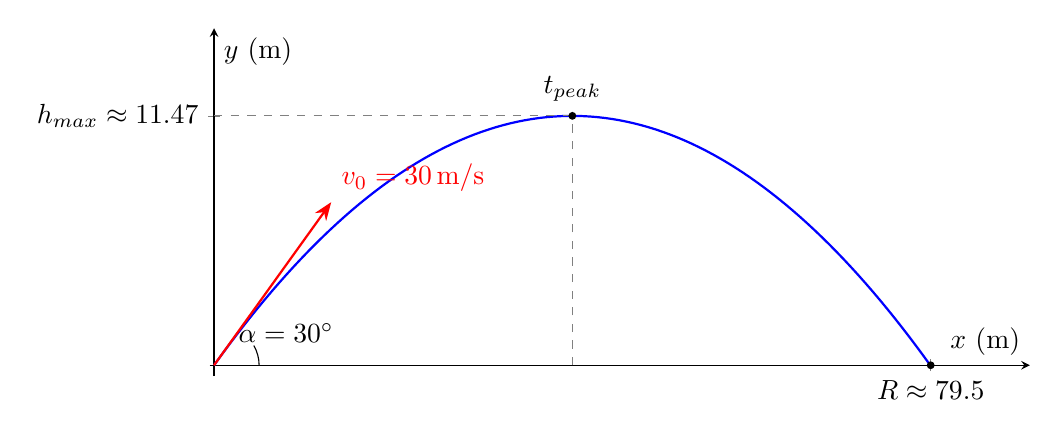
\begin{tikzpicture}[>=Stealth,thick]
\begin{axis}[
    axis lines = middle,
    xlabel = {$x$ (m)},
    ylabel = {$y$ (m)},
    xmin = 0, xmax = 90,
    ymin = 0, ymax = 15,
    width=12cm, height=6cm,
    xtick={0, 79.5},
    xticklabels={0, $R \approx 79.5$},
    ytick={11.47},
    yticklabels={$h_{max} \approx 11.47$},
    grid = none,
    enlargelimits={abs=0.5}
]
    % Pályagörbe rajzolása (y = x*tan(30) - g*x^2 / (2 * v0^2 * cos(30)^2))
    \addplot [
        domain=0:79.5, 
        samples=100, 
        color=blue,
        thick,
    ] {x*tan(30) - (9.81*x^2)/(2*30^2*cos(30)^2)};

    % Kezdősebesség vektor (v0)
    \draw[->, thick, red] (axis cs:0,0) -- (axis cs:13, 7.5) node[above right] {$v_0 = 30\,\text{m/s}$};
    
    % Szög jelölése
    \draw (axis cs:5,0) arc [start angle=0, end angle=30, radius=5mm];
    \node at (axis cs:8, 1.5) {$\alpha=30^\circ$};

    % Maximum magasság jelölése szaggatott vonallal
    \draw[dashed, gray] (axis cs:39.75, 0) -- (axis cs:39.75, 11.47);
    \draw[dashed, gray] (axis cs:0, 11.47) -- (axis cs:39.75, 11.47);
    \node[circle, fill=black, inner sep=1pt, label=above:{$t_{peak}$}] at (axis cs:39.75, 11.47) {};

    % Hatótávolság pontja
    \node[circle, fill=black, inner sep=1pt, label=below right:{$t_{total}$}] at (axis cs:79.5, 0) {};
\end{axis}
\end{tikzpicture}
\end{center}

\vskip -40 pt

\begin{enumerate}
\item Vertical velocity component: $v_{0y} = v_0 \sin\alpha = 30 \cdot \sin(30^\circ) = 15\,\text{m/s}$.  \\ Time to reach the peak: $t_{peak} = \frac{v_{0y}}{g} = \frac{15}{9.81} \approx 1.53\,\text{s}$.
\item Maximum height: $h_{max} = \frac{v_{0y}^2}{2g} = \frac{15^2}{2 \cdot 9.81} \approx 11.47\,\text{m}$
\setcounter{enumii}{3}  
\item Total time of flight: $t_{total} = 2 \cdot t_{peak} \approx 3.06\,\text{s}$.
\setcounter{enumii}{2}  
\item Horizontal range: $R = v_0 \cos\alpha \cdot t_{total} = 30 \cdot \cos(30^\circ) \cdot 3.06 \approx 79.50\,\text{m}$.
\end{enumerate}

% ------------------------------------------------------------------------------------------------

\item At what distance from the Mars does an areosynchronous satellite orbit in the plane of the Equator if it remains constantly above the same point on the Mars's surface?

\smallskip

\begin{center}
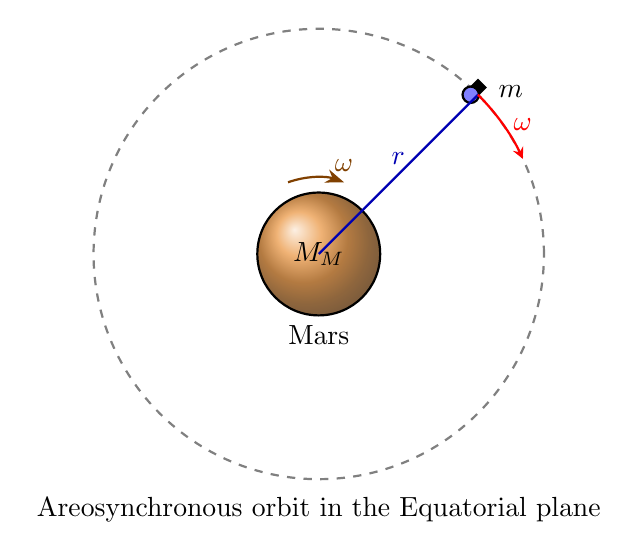
\begin{tikzpicture}[scale=1.3,>=Stealth,thick]
    % Mars (at center)
    \shade[ball color=orange!60!brown, opacity=0.8] (0,0) circle (0.6);
    \draw[thick] (0,0) circle (0.6);
    \node at (0,0) {$M_M$};
    \node[below] at (0,-0.6) {Mars};

    % Areosynchronous orbit (dashed line)
    \draw[dashed, gray] (0,0) circle (2.2);

    % Satellite (m) on the orbit
    \begin{scope}[rotate=45]
        \draw[fill=black] (2.2,0) rectangle (2.3,0.1); % Solar panels
        \draw[fill=black] (2.1,0) rectangle (2.2,0.1);
        \draw[fill=blue!50] (2.15, 0.05) circle (0.08); % Satellite body
        \node[right=5pt] at (2.2, 0.05) {$m$};
        
        % Radius (r) indication
        \draw[-, >=stealth, thick, blue!70!black] (0,0) -- (2.2,0) node[midway, above, sloped] {$r$};
        
        % Angular velocity direction
        \draw[->, >=stealth, thick, red] (2.2,0.0) arc[start angle=0, end angle=-20, radius=2.2] node[midway, right] {$\omega$};
    \end{scope}

    % Rotation of Mars
    \draw[->, thick, orange!50!black] (-0.3,0.7) arc[start angle=110, end angle=70, radius=0.8] node[above] {$\omega$};

    % Caption
    \node at (0,-2.5) {Areosynchronous orbit in the Equatorial plane};
\end{tikzpicture}
\end{center}

\vskip -30 pt
\begin{eqnarray*}
G \frac{M_{M} m}{r^2} &=& m \omega^2 r = m \left(\frac{2\pi}{T}\right)^2 r  \\
  r &=& \sqrt[3]{\frac{G M_M T^2}{4\pi^2}}  \\
\end{eqnarray*}
\vskip -25 pt
The mass of Mars is $M_M \approx 6.417 \cdot 10^{23}\,\text{kg}$, and its rotation period is $T \approx 24.62\,\text{h} = 88642\,\text{s}$. Therefore, $$r = \sqrt[3]{\frac{6.674 \cdot 10^{-11} \cdot 6.417 \cdot 10^{23} \cdot 88642^2}{4\pi^2}} \approx 2.04 \cdot 10^7\,\text{m} \approx 20400\,\text{km}.$$ Finally, $h=20400\,\text{km}-3390\,\text{km}=17010\,\text{km}$.

% ------------------------------------------------------------------------------------------------

\pagebreak
\item A $2\,\text{kg}$ object slides down from the top of a $3\text{-meter-high}$ inclined plane that makes an angle of $30^\circ$ with the horizontal. What is the velocity of the object when it reaches the bottom of the incline, starting from rest at the top, if:
\begin{enumerate}
    \item[(a)] there is no friction between the object and the incline?
    \item[(b)] the coefficient of friction is $0.05$?
\end{enumerate}

\smallskip

\begin{center}
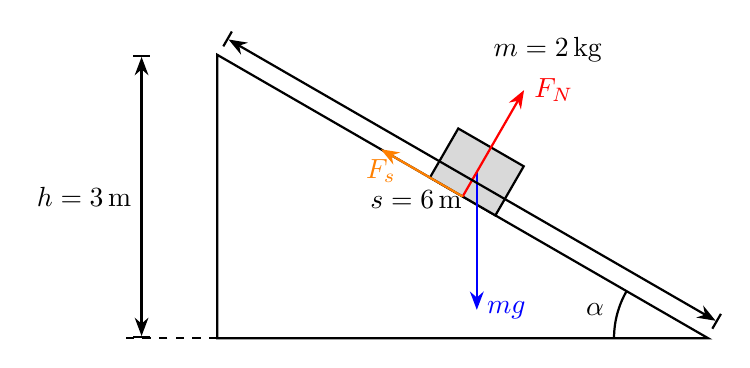
\begin{tikzpicture}[scale=1.2,>=Stealth,thick]
    % Változók definiálása
    \def\angle{30}
    \def\height{3}
    \def\length{6} % s = h / sin(30) = 6
    \def\base{5.196} % s * cos(30)
    
    % Lejtő megrajzolása
    \draw (0,0) coordinate (B) -- (\base,0) coordinate (C) -- (0,\height) coordinate (A) -- cycle;
    
    % Vízszintes segédvonal a szögnek (ha másho1gy akarjuk jelölni)
    \draw[dashed] (0,0) -- (-1,0);
    
    % Szög jelölése
    \draw (4.2,0) arc (0:-30:-1);
    \node at (4.0,0.3) {$\alpha$};

    % A test (téglalap a lejtőn)
    \begin{scope}[shift={(0.5*\base, 0.5*\height)}, rotate=-\angle]
        \draw[fill=gray!30] (-0.4,0) rectangle (0.4,0.6);
        \node at (0.0, 1.8) {$m = 2\,\text{kg}$};
        
        % Erők (opcionális, de szemléletes)
        \draw[->, blue,rotate=\angle] (0.15,0.26) -- (0.15,-1.2) node[right] {$mg$}; % Súlyerő
        \draw[->, red] (0,0.0) -- (0,1.3) node[right] {$F_N$}; % Tartóerő
        \draw[->, orange] (0,0) -- (-1,0) node[below] {$F_s$}; % Súrlódás (ha van)
    \end{scope}

    % Méretek jelölése
    \draw[|<->|] (-0.8,0) -- node[left] {$h = 3\,\text{m}$} (-0.8,\height);
    \draw[|<->|] ({0.2*sin(\angle)}, {\height + 0.2*cos(\angle)}) -- node[below left] {$s = 6\,\text{m}$} ({\base + 0.2*sin(\angle)}, {0.2*cos(\angle)});
\end{tikzpicture}
\end{center}

\vskip -30 pt
\begin{enumerate}
\item There is no friction between the object and the incline: $$mgh = \frac{1}{2}mv_a^2 \implies v_a = \sqrt{2gh} = \sqrt{2 \cdot 9.81 \cdot 3} \approx 7.67\,\text{m/s}$$
\item $\mu=0.05$
\vskip -30 pt
\begin{eqnarray*}
s &=& \frac{h}{\sin\alpha} = \frac{3}{\sin 30^\circ} = 6\,\text{m}  \\
W_{fric} &=& \mu F_N s = \mu (mg \cos\alpha) s  \\
mgh - \mu mg \cos\alpha \cdot s &=& \frac{1}{2}mv_b^2  \\
v_b &=& \sqrt{2g(h - \mu s \cos\alpha)} = \sqrt{2 \cdot 9.81 \cdot (3 - 0.05 \cdot 6 \cdot \cos 30^\circ)} \approx 7.33\,\text{m/s} 
\end{eqnarray*}
\end{enumerate}


% ------------------------------------------------------------------------------------------------

\item A string is wound around a solid cylinder with radius $R = 0.5\,\text{m}$ and mass $M = 30\,\text{kg}$. Two objects with a combined mass of $15\,\text{kg}$ are hanging from the ends of the string. Upon release, the cylinder accelerates with an angular acceleration of $\beta = 4\,\text{rad/s}^2$. The string does not slip.
\begin{itemize}
    \item[(a)] Find the individual masses ($m_1, m_2$) of the two objects.
    \item[(b)] Calculate the total kinetic energy of the system at $t = 4\,\text{s}$.
\end{itemize}

\smallskip
\begin{center}
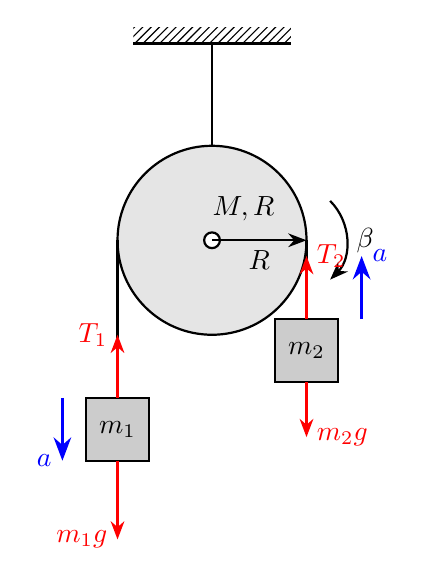
\begin{tikzpicture}[>=Stealth, thick,scale=1.0]
    % Plafon (felfüggesztés)
    \fill[pattern=north east lines] (-1,2.5) rectangle (1,2.7);
    \draw (-1,2.5) -- (1,2.5);
    
    % Csiga felfüggesztése
    \draw (0,2.5) -- (0,0.5);
    
    % Csiga (Henger)
    \def\R{1.2} % Sugár a rajzon
    \draw[fill=gray!20] (0,0) circle (\R);
    \draw[fill=white] (0,0) circle (0.1); % Tengely
    
    % Feliratok a csigához
    \node at (0.4, 0.4) {$M, R$};
    \draw[->] (0,0) -- (\R,0) node[midway, below] {$R$};
    \draw[->, bend left=45] (1.5,0.5) to node[right] {$\beta$} (1.5,-0.5);

    % Kötél és tömegek
    % m1 (nehezebb, bal oldalon lefelé mozog)
    \draw (-\R, 0) -- (-\R, -2);
    \draw[fill=gray!40] (-\R-0.4, -2) rectangle (-\R+0.4, -2.8);
    \node at (-\R, -2.4) {$m_1$};
    \draw[->, blue, very thick] (-\R-0.7, -2) -- ++(0,-0.8) node[left] {$a$};

    % m2 (könnyebb, jobb oldalon felfelé mozog)
    \draw (\R, 0) -- (\R, -1);
    \draw[fill=gray!40] (\R-0.4, -1) rectangle (\R+0.4, -1.8);
    \node at (\R, -1.4) {$m_2$};
    \draw[->, blue, very thick] (\R+0.7, -1) -- ++(0,0.8) node[right] {$a$};

    % Erők m1-en
    \draw[->, red] (-\R, -2) -- (-\R, -1.2) node[left] {$T_1$};
    \draw[->, red] (-\R, -2.8) -- (-\R, -3.8) node[left] {$m_1g$};

    % Erők m2-n
    \draw[->, red] (\R, -1) -- (\R, -0.2) node[right] {$T_2$};
    \draw[->, red] (\R, -1.8) -- (\R, -2.5) node[right] {$m_2g$};
\end{tikzpicture}
\end{center}

\begin{enumerate}
\item Masses:
\vskip -30 pt
\begin{eqnarray*}
a &=& \beta R = 4 \cdot 0.5 = 2\,\text{m/s}^2  \\
  \tau &=& (T_1 - T_2)R = I\beta = \left(\frac{1}{2}MR^2\right)\beta \implies T_1 - T_2 = \frac{1}{2}MR\beta  \\
\end{eqnarray*}
\begin{eqnarray*}
  m_1g - T_1 &=& m_1a, \quad T_2 - m_2g = m_2a \implies \\
   T_1 &=& m_1(g-a), \ T_2 = m_2(g+a)  \\
  m_1(g-a) - m_2(g+a) &=& \frac{1}{2}MR\beta  \\
m_1 + m_2 &=& 15 \implies m_2 = 15 - m_1  \\
m_1(9.81-2) - (15-m_1)(9.81+2) &=& \frac{1}{2} \cdot 30 \cdot 0.5 \cdot 4 = 30  \\
  7.81m_1 - 177.15 + 11.81m_1 &=& 30 \implies 19.62m_1 = 207.15  \\
\end{eqnarray*}
\vskip -50 pt
$$m_1 \approx 10.56\,\text{kg}, \ m_2 \approx 4.44\,\text{kg}$$
\vskip -30 pt
\item Total kinetic energy:
\vskip -30 pt
\begin{eqnarray*}
\omega &=& \beta t = 4 \cdot 4 = 16\,\text{rad/s}, \quad v = \omega R = 16 \cdot 0.5 = 8\,\text{m/s}  \\
E_{kin} &=& \frac{1}{2}I\omega^2 + \frac{1}{2}(m_1+m_2)v^2 = \frac{1}{4}MR^2\omega^2 + \frac{1}{2}(15)v^2  \\
E_{kin} &=& \frac{1}{4} \cdot 30 \cdot 0.5^2 \cdot 16^2 + 0.5 \cdot 15 \cdot 8^2 = 480 + 480 = 960\,\text{J} 
\end{eqnarray*}
\end{enumerate}

% ------------------------------------------------------------------------------------------------

\item Estimate the average depth of the Pacific Ocean if a tsunami takes 5 hours to travel from Hawaii to Alaska. (Note: The propagation speed of shallow-water waves is $v=\sqrt{gh}$. The distance is $4000$\,km.)

\smallskip
\begin{center}
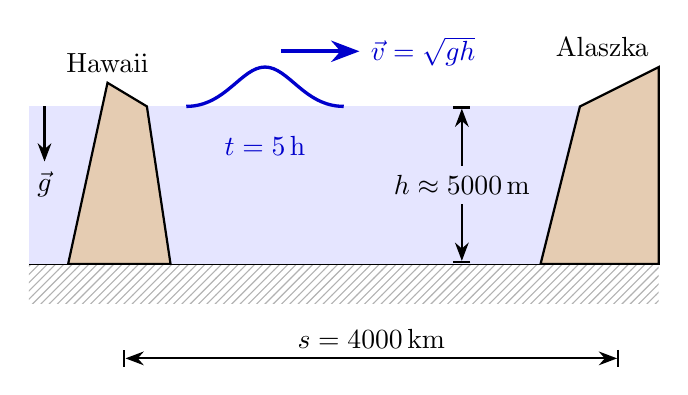
\begin{tikzpicture}[>=Stealth, thick]
    % Koordináták definiálása
    \def\oceanWidth{8}
    \def\oceanDepth{2}
    \def\wavePos{3}

    % Óceánfenék (minta)
    \fill[pattern=north east lines, pattern color=gray!60] (0,-0.5) rectangle (\oceanWidth,0);
    \draw (0,0) -- (\oceanWidth,0);

    % Vízfelület és víztest
    \fill[blue!10] (0,0) rectangle (\oceanWidth,\oceanDepth);
    
    % Hawaii (Sziget)
    \draw[fill=brown!40] (0.5,0) -- (1, \oceanDepth+0.3) -- (1.5, \oceanDepth) -- (1.8,0) -- cycle;
    \node[above] at (1, \oceanDepth+0.3) {Hawaii};

    % Alaszka (Partvonal)
    \draw[fill=brown!40] (\oceanWidth-1.5, 0) -- (\oceanWidth-1, \oceanDepth) -- (\oceanWidth, \oceanDepth+0.5) -- (\oceanWidth, 0) -- cycle;
    \node[above left] at (\oceanWidth, \oceanDepth+0.5) {Alaszka};

    % Hullám (Tsunami)
    \draw[blue!80!black, very thick] 
        (\wavePos-1, \oceanDepth) .. controls (\wavePos-0.5, \oceanDepth) and (\wavePos-0.3, \oceanDepth+0.5) .. 
        (\wavePos, \oceanDepth+0.5) .. controls (\wavePos+0.3, \oceanDepth+0.5) and (\wavePos+0.5, \oceanDepth) .. 
        (\wavePos+1, \oceanDepth);
    
    % Sebesség vektor
    \draw[->, blue!80!black, ultra thick] (\wavePos+0.2, \oceanDepth+0.7) -- ++(1,0) node[right] {$\vec{v} = \sqrt{g h}$};

    % Mélység jelölése (h)
    \draw[|<->|] (5.5, 0.01) -- node[fill=blue!10] {$h \approx 5000\,\text{m}$} (5.5, \oceanDepth);

    % Távolság jelölése (s)
    \draw[|<->|] (1.2, \oceanDepth-3.2) -- node[above] {$s = 4000\,\text{km}$} (\oceanWidth-0.5, \oceanDepth-3.2);

    % Idő felirat
    \node[blue!80!black] at (\wavePos, \oceanDepth-0.5) {$t = 5\,\text{h}$};
    
    % Gravitációs vektor
    \draw[->] (0.2, \oceanDepth) -- (0.2, \oceanDepth-0.7) node[below] {$\vec{g}$};

\end{tikzpicture}
\end{center}

\vskip -10 pt
\begin{eqnarray*}
v &=& \frac{s}{t} = \frac{4000000\,\text{m}}{5 \cdot 3600\,\text{s}} \approx 222.22\,\text{m/s}  \\
v &=& \sqrt{gh} \implies h = \frac{v^2}{g}  \\
h &=& \frac{222.22^2}{9.81} \approx 5034\,\text{m} 
\end{eqnarray*}

\end{enumerate}

% ------------------------------------------------------------------------------------------------

\bigskip

\rightline{Dr.~Gabor~FACSKO}
\rightline{\textit{facsko.gabor@uni-obuda.hu}}

\vfill

\end{document}
